%!TEX root = ../Thesis.tex
\chapter{Diabetes Type-2 and Oral Insulin}


\textit{"Diabetes is one of the first diseases described in an Egyptian manuscript from c. 1500 BCE mentioning "too great emptying of the urine." The first described cases are believed to be type 1 diabetes. Indian physicians around the same time identified the disease and classified it as madhumeha or honey urine, noting that the urine would attract ants. The term "diabetes" or "to pass through" was first used in 230 BCE by the Greek Apollonius Of Memphis. The disease was rare during the time of the Roman empire with Galen commenting that he had only seen two cases during his career. Type 1 and type 2 diabetes were identified as separate conditions for the first time by the Indian physicians Sushruta and Charaka in 400–500 AD with type 1 associated with youth and type 2 with being overweight. The term "mellitus" or "from honey" was added by the Briton John Rolle in the late 1700s to separate the condition from diabetes insipidus which is also associated with frequent urination. Effective treatment was not developed until the early part of the 20th century when the Canadians Frederick Banting and Charles Best discovered insulin in 1921 and 1922. This was followed by the development of the long acting NPH insulin in the 1940s."}

-\url{https://en.wikipedia.org/wiki/History_of_diabetes} \footnote{I dedicate this first quotation to Wikipedia a community curated encyclopedia. Open and free communities such as stackexchange.com (cross validated, stack-overflow, Tex, ...), R mailing list, youtube.com have taught me the most in the last three years. I hope scientific literature, soon also will become open source. That means open access to content and also a transparent community driven editing and reviewing process unlike today.}
\newpage

\section{Diabetes}
Diabetes is a major challenge to general health and quality of life in almost every country world wide. Type-2 accounts for the most incidents of diabetes and is strongly associated with lack of physical exercise, an unfavorable diet and obesity. Other risk factors are age and genetic predispositions. Type-2 diabetes is not only a problem in industrialized countries.  World-wide 380 million people are estimated to be affected and 15\% of deaths are attributable to diabetes. \cite{aguiree2013idf}.


\subsection{Blood sugar regulation in diabetic and healthy patients}
Type-1 diabetes  is defined as the inability to produce insulin due to the not fully understood auto-immune rejection of the insulin producing beta-cells. The typical onset of Type-1 diabetes is at child age or youth. Insulin is an important hormone for regulation of the human metabolism, as it promotes uptake of glucose in the liver, muscles and fat tissue. An oscillating level of insulin is required to regulate the energy metabolism during the day. Shortly after a meal, insulin is released to signal the start of glucose take up. In fasting state, insulin levels in healthy persons are low, as no new glucose is obtained from digestion. Insulin has an oppositely acting counterpart, glucagone, that promotes release of glucose primarily from the liver. Type-2 diabetes is defined by insulin resistance, where the peripheral tissues and the liver do not respond sufficiently to the endogenously produced insulin. When blood glucose levels exceeds 10 mmol/L (180 mg/dL), the kidney can no longer re-uptake all glucose from the excreted urine. The glucose in urine will sequentially increase osmolality and prevent the kidney from also reabsorbing water and hence the higher rate of sweet urine and the name diabetes mellitus. A healthy human can regulate the blood sugar within 3.9 mmol/L and 7.8 mmol/L throughout a normal day cycle. After the meals of the day, the food is metabolized and free glucose comes into blood circulation. Without regulation, a single meal would make the blood sugar far exceed normal levels\cite{silverthorn2010human,Cowart1990}.

To put these numbers in to perspective, ideally elevating the blood glucose from 3.9 to 7.8 mmol/L for adult of 80 kg and 8 liters of blood would only require
$ \frac { (7.8-3.9) \textrm{mmol/L} \quad 180\textrm{mg/dL} }
		{ 10 \textrm{mmol/L} } = 5.3 \textrm{g}$ of glucose.

The pancreas, located adjacent to the first part of the intestine after the stomach, senses systemic blood sugar levels. The pancreas can also receive hormone signaling from the adjacent small intestines (e.g. GLP-1), indicating that food currently is being metabolised and systemic blood sugar soon will rise. Thus, whenever needed under and after a meal, the pancreas will release insulin. Insulin triggers a number of blood glucose lowering responses, rendering cellular uptake and storage of glucose. Glucose is stored short-term in the liver and muscles and in part converted to fat and stored long-term in fatty tissues. The liver is the major short term energy storage, taking up glucose and converting it to polymeric glucogen, that when needed can be reconverted into glucose and released to systemic circulation again. For type-2 patients, insulin secretion is constantly elevated to compensate for the insulin resistance, and therefore the pancreas cannot further regulate the glucose load from a meal, as it is already producing insulin almost as fast as possible \cite{silverthorn2010human}. With a long-acting insulin analogue for a type-2 diabetic, the insulin requirement from the pancreas is no longer maxed out, such that the pancreas again can up and down regulate the insulin level during the day.

\begin{figure}[!htpb]
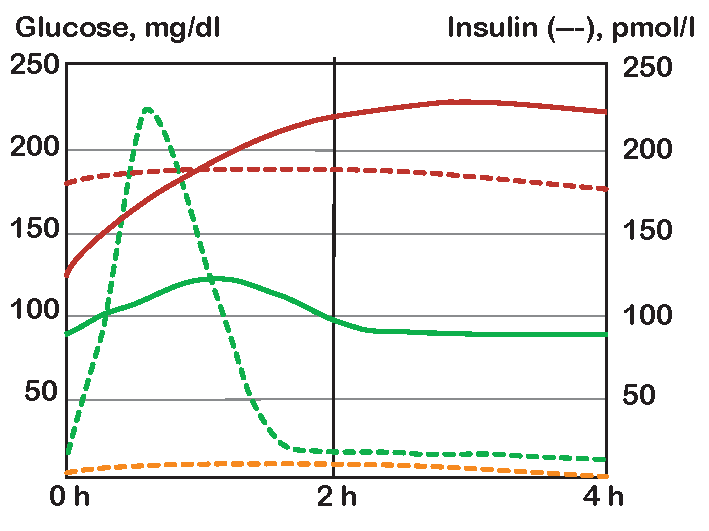
\includegraphics[width=0.8\textwidth,height=0.8\textheight,keepaspectratio]{graphics/glucoseTolerance.pdf}
\caption{Glucose tolerance test: A typical healthy patient has a very low fasting insulin level (dashed green line) and a high transient response to regulate a glucose intake at 0 hours. A healthy patient is able to lower glucose level within 2 hours after glucose intake (green line). The insulin level of an untreated Type-2 patient (red dashed line) is already elevated and no further compensation is possible. The glucose level (red line) will not stabilize within 2 hours. Yellow dashed line represents a Type-1 patient with almost no endogenous insulin production. If untreated, glucose levels would exceed the ranges of this axis. Figure is reproduced by redrawing and combining illustrations from \cite{silverthorn2010human,caumo2004first}}
\label{glucoseTolerance}
\end{figure}

A glucose tolerance test is used to diagnose diabetes. Figure \ref{glucoseTolerance} outlines a glucose tolerance test and the response from a healthy subject as well as for a type-1 and type-2 diabetic patient. A type-1 diabetic patient will have no endogenous regulation of blood sugar and both long acting and well timed short acting insulin therapy is needed. However, due to uncertainties of timing and variance of bio-availability, oral insulin therapy can only substitute long-acting insulin. As type-1 diabetics are already treating themselves with injectable short-acting insulin in conjunction with meals, there is little rationale in replacing their long-acting basal insulin injectable formulation with an oral tablet formulation. In contrary for type-2 diabetics that only need a basal long acting insulin therapy to assist their pancreas in regulating the blood glucose, an oral insulin therapy would be a convenient option to have.





\subsection{Treatment and compliance}
Intensive anti-diabetic therapy is important to avoid or delay myocardial infarct, micro vascular diseases and kidney related complications \cite{holman,boussageon2011effect,gaede2008effect}. Having a chronic elevated high blood glucose level is simply very unhealthy long-term and will reduce the quality of life. As the type-2 diabetes progresses, glyceamic control is no longer achievable with a single oral agent such as Metformin or Sulfonylurea, which receptively lowers insulin resistance and increases endogenous insulin production. Injectable peptide based formulations of insulin-analogues or GLP-1-analogues will inevitably be considered at some point in the disease stage progression. Inconvenience and patient compliance are the main factors for not achieving the clinical recommendations for blood glucose control in insulin treatment of type II diabetes patients. To initiate injectable insulin therapy is a psychological barrier for Type-2 patients and a cause of worrying \cite{korytkowski2002oral}. Nevertheless insulin therapy will eventually become the outcome for most Type-2 patients. From early onset type-2 patients still have the ability to regulate blood sugar to some level and strict hourly control is not needed. In two groups of 24,000 and 10,000 patients of seniors aged 60-69, the former group was diagnosed with type-2 diabetes within last 9 years and the latter group has been diagnosed more than 9 years ago. When recently diagnosed, patients are prescribed oral hypoglycaemic agents (OHA). Therefore 50\% of early diagnosed patients received metformin and/or sulfonylurea. Only 7.5\% received insulin treatment. In contrast, in patients diagnosed more than 9 years ago, fully 65\% are ordinated treatments based on injectable insulin \cite{Elbert2014rates}. Thus a typical type-2 diabetes disease progression will start with fairly convenient once a day tablets, mildly lowering glucose. Hereby the constant insulin production of the pancreas is lowered, giving the pancreas a insulin buffer capacity to regulate blood glucose throughout the day. With time, more insulin is needed to obtain sufficient blood glucose control. The disease will progress from a treatment only complimenting the anatomical blood sugar regulating mechanisms, to the insulin therapy becoming the main regulation of blood glucose.

Compliance is the extent of which the patient uses the medicine as prescribed by the physician. Especially for short acting injectable insulins, daily awareness and monitoring of blood glucose and storing injectable insulin refrigerated may be a large requirement for the patient. Type-1 patients who came to master these skills early in life, are likely to have a much higher compliance. Simply, the patient must learn to live by a fairly complex treatment regimen late in life. Compliance for only oral agents can already be as low is 50\% after six months \cite{garcia2013adherence}. In a study 50\% of insulin-naive patients perceived injectable insulin initiation as a failure. In a study of those patients who did not comply to an treatment regime with injectable insulin, the most common reasons given were planing to improve healthy behavior instead (25\%), fear of injection (13\%), negative impact on work (9\%), concerns on long term medication (9\%), inconvenience (6\%), and not believing insulin was necessary (6\%). Despite the various available anti diabetic agents for various stages of type-2 diabetes, it is indicated that less than 50\% of patients achieve the aimed glucose control recommended and around two-thirds will die prematurely of cardiovascular disease \cite{garcia2013adherence}. In contrary it is argued that current injection pens actually have improved comfort for insulin injection so much, that needle phobia alone is not at strong argument for developing oral insulin formulations \cite{maher2014formulation}.

The possible introduction of oral insulin may provide a mid-way solution, especially for type-2 patients where other oral agents no longer are potent enough, yet with the same ease of administration as oral agents. Thus oral insulin may prolong the time the patient can regulate blood sugar without injectable insulin and perhaps improve compliance.

\section{Drug Development Challenges of Oral Insulin}
Oral formulations of insulin is not an obviously great idea. One broad intuitive explanation is: From natures side, an organism tend not take up any foreign substances, and certainly not foreign proteins or peptides. External proteins and peptides are likely produced by foreign species, and therefore have been created to serve independent purposes, that not necessarily are in alignment with the survival of this organism.

Likewise, the human body has a series of barriers in the gastrointestinal tract before proteins such as insulin, reach systemic circulation. Figure \ref{intro_anatomy} illustrates the upper gastrointestinal tract and the barriers for insulin.

\begin{figure}[!htbp]
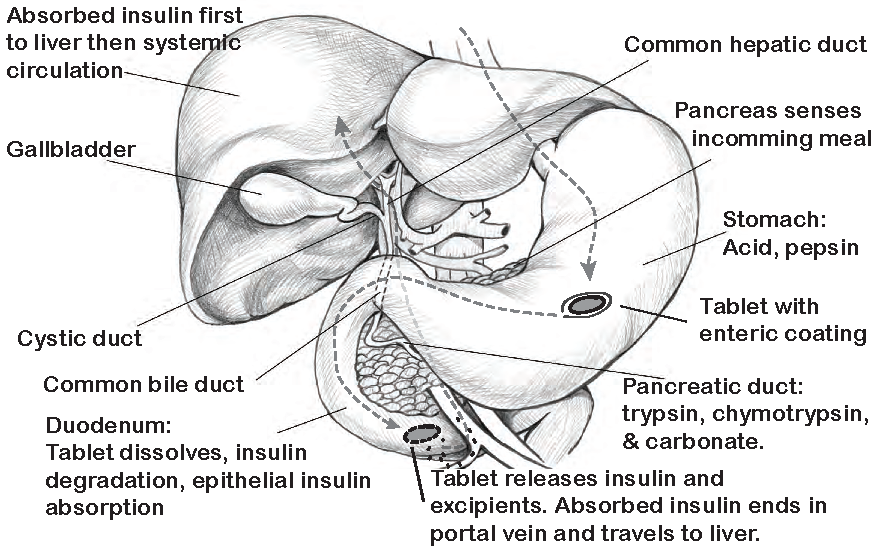
\includegraphics[width=\textwidth,height=\textheight,keepaspectratio]{graphics/intro_anatomy2.pdf}
\caption{(1) Tablet coating protects against acidic hydrolysis and pepsin. (2) Release of basic carbonate, bile, trypsin and chymotrypsin. Pepsin is inactivated at neutral pH. Bile interferes with surfactant like absorption enhancers. (3) Tablet dissolves. Lipophilic absorption enhancers will slow down insulin release and allow trypsin and chymotrypsin to inactivate all insulin before absorption. (4) Insulin permeates duodenal and jenunal epithelia facilitated by absorption enhancers. Illustration kindly provided for public use by NIH: National Institute of Diabetes and Digestive and Kidney Diseases. \url{https://catalog.niddk.nih.gov/imagelibrary/detail.cfm?id=148} Original captions modified.}
\label{intro_anatomy}
\end{figure}


\subsection{Acid resistant coating}
 Normal protein digestion starts in the stomach with the enzyme pepsin cleaving protein amide-bonds next to lipophilic/aromatic amino acids. Insulin formulations are simply protected towards pepsin and acidic hydrolysis with an acid insoluble tablet coating. The coating is made of polymers with pH-dependent solubility. Acidic side groups will only deprotonate under neutral pH. Deprotonation, and hence ionization, increases the solubility of the otherwise non-ionic lipophilic polymers \cite{carino1999oral,gabor2010improving}. Most coatings are designed to dissolve at pH > 5.5 \cite{maher2014formulation}.
 
The sphincther, the opening muscle of the stomach, forwards some of the acidic stomach content to the upper duodenum and eventually the coated tablet or capsule. The insulin producing gland, the pancreas, is central to the gastro intestinal digestion. The pancreas will secrete to the pancreatic duct alkaline carbonate to neutralize the hydrochloric stomach acid. The stomach enzyme pepsin is deactivated by neutral pH, while neutral acting trypsin and chymotrypsin are released from the pancreas as well. Depending on the thickness and the acid groups of the coating polymer, the tablet/capsule will start dissolving immediately in the duodenum and jejunum or as late as in the colon.

The stomach empties approximately only every 50-120 minutes during fasting and even rarer for diabetic patients \cite{silverthorn2010human,corvilain1995effect,gabor2010improving}, thus the accuracy of timing of the dose is not likely to match injectable insulin. Therefore, oral insulin is not likely to replace fast acting well timed doses of injectables used by type-1 diabetics in connection with meals. Oral insulin is most likely to replace longer acting insulin analogues, where the exact onset of action is of less concern.

\subsection{The peptide itself: Size does matter, so does lasting long and stability}
Presently several oral insulin formulations are in clinical phase two and three. These formulations can rely on a protein backbone modification to make insulin intrinsically more stable to enzymatic degradation. The formulations' approaches to increase the bio-availability are: absorption enhancers, enzyme inhibitors (soybean, citric acid) and micro/nano-encapsulated carriers \cite{aguirre2016current}. Oral delivery of other peptides such as glukagon-like peptide-1 (GLP-1) analogues, octreotide (somatostain agonist), parathyroid hormone are also in clinical development in 2016 \cite{aguirre2016current}.

Peptide APIs in oral formulations targeting systemic circulation, that have been approved by FDA or EMA are Cyclosporin (MW 1200) Desmopressin (MW 1100), Taltirelin (MW 500) and glutathione (MW 300) \cite{aguirre2016current}. The reason these four APIs have been successfully introduced to market before insulin is likely in part their significantly smaller size than monomeric insulin (MW 6000) and these peptides can therefore permeate the epithelial barrier more easily. With the current formulation technology it is only barely possible to administer insulin.
\begin{quote}
"The selection of a suitable peptide for oral formulation is, therefore, a key commercial decision. For example, selecting a complex, high molecular weight (MW), narrow therapeutic index peptide, manufactured by a costly recombinant approach, requiring multiple daily oral administrations would be problematic."
\cite{maher2014formulation}
\end{quote}

In this quote, Maher \textit{et al} point out that oral peptide delivery for decades has been in its infancy and that we cannot suddenly deliver any type of peptide. In fact the current achievements are more attributable to the biotechnological advances allowing modification of the peptide and cheap production. If less than 5\% insulin is absorbed, 20 times as much insulin must be produced.

Treatment with injectable peptides such as insulin, GLP-1 and growth hormone have become more convenient with fewer injections in the last decades, as extensive research has aimed to modify the intrinsic endogenous hormone to increase the apparent and actual half-life. The apparent half-life is extended by formulation approaches only gradually releasing the insulin from the injection site, but also the systemic half-life can be extended \cite{arnolds2010pharmacokinetic}. Hereby, patients treated with a constant level of hormone, only have to inject themselves daily or even weekly. Oral peptide formulations at first will likely be attempted switches from their prenatally-marketed counterparts \cite{maher2014formulation}. As only a couple of percentages of the peptides are likely absorbed, the relative variation of absorption is potentially very high \cite{gabor2010improving}. A dosing interval significantly shorter than the half-life of the drug is a classic method for maintaining a relatively constant drug concentration within the therapeutic window \cite{tozer2006introduction}.

Analogues with enzymatic stability are also required. The luminal enzyme activity by trypsin and chymotrypsin will likely inactivate released insulin in less than 5-15 minutes \cite{welling2014citric}. Co-formulation of soy-bean enzyme inhibitors \cite{fujii1985promoting}, covalent peptide protecters (SNAC) \cite{bruno2013basics} and pH lowering \cite{welling2014citric} can only lower degradation 2 to 5-fold. Designing stable analogues is also needed to obtain sufficient stability. PEGylation, cyclization and modification of back-bone structure are known approaches to increase intrinsic peptide analogue stability \cite{bruno2013basics}.

\subsection{Permation enhancers to open the epithelial barrier}
Thirdly peptides or proteins have to pass the epithelial barrier. Insulin (MW 6000 D) is likely near the upper limit for how big the proteins currently can be successful delivered. For Octertide, it was possible to select a small part of the peptide while still retaining activity \cite{aguiree2013idf}. 

Fatty acids with C8 to C16 chains have been used to open tight junction between epithelial cells and mildly perturb the phospholipid membrane of the epithelials cells. There has been an extensive research \cite{bruno2013basics,maher2009safety,artursson1990epithelial} uncovering how caprate (aka. C10) regulate calcium levels, and phosphyrolation cascades of the epithelial cells leading to opening of tight junctions. Nonetheless, in order to obtain a sufficient response caprate has to be released in intestinal lumen in concentrations close to the critical micelle contration which is where the perturbing effect on the phospholipid membrane sets in \cite{bruno2013basics}. No specific technology increasing protein absorption significantly has emerged from the caprate-calcium-tight junction-theory. In practice fatty acids are surfactants, and most surfactants will destabilize the epithelial membrane and promote peptide absorption. The important part is how wide is the therapeutic window, potency versus toxicity and if these surfactant ate sufficiently soluble. I do not dismiss that, biological effects such as the C10-Calcium-tight junctions in theory may render one surfactant slightly more or less potent. However, such effects would be difficult to predict, see Section \ref{modelComplexity}. The working hypothesis of this thesis is that central properties of surfactants are fairly possible to predict as they arise from non-complex physical phenomena, and new absorption enhancers could be discovered simply from the expected structure. In contrary it is not possible to learn the mechanism of receptor mediated permeation enhancers, as even the smallest change in the molecule could change the receptor-agonist affinity.

Where fatty acids have one deprotonated carboxylic acid as hydrophile head group, there several other possible head groups. Most enhancers have a mono acyl chain typically from 8 to 16 carbon atoms and some hydrophilic domaine. Other surfactant enhancer classes are e.g. the acyl-carnitines, acyl-cholates\cite{lee2000oral}, phosphocholines\cite{liu1999dodecylphosphocholine}, acyl-maltosides \cite{petersen2013colonic} and acyl sulphates \cite{anderberg1993epithelial}.

